% !TEX root = ./main.tex
\section{Supplementary Files}
\label{sec:SI_files}
\begin{itemize}
    \item Plasmid Sequences with annotations + RiboJ::YFP
    \item pHelper sequence
    \item Primers
    \item list of restriction sites used in cloning
    \item Gene list
    \item Sequencing Data
    \item List of ordered sequences
\end{itemize}

\clearpage

\section*{Supplementary Figures}
\begin{figure}[H]
    \centering
    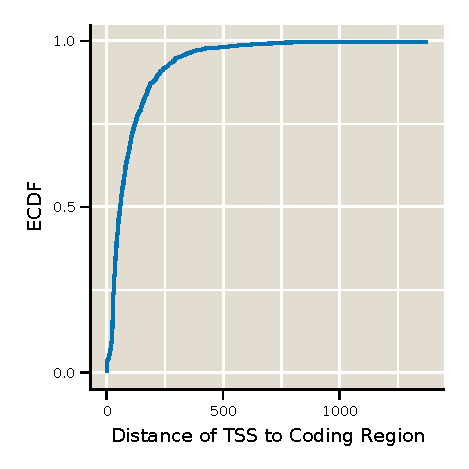
\includegraphics{../figures/tss_CR_distance.pdf}
    \caption{ECDF of distances of transcription start sites to the coding region for every operon in \textit{E. coli} that has a transcription start site annotated in EcoCyc. }
    \label{fig:tss_distance}
\end{figure}


\begin{figure}[H]
    \centering
    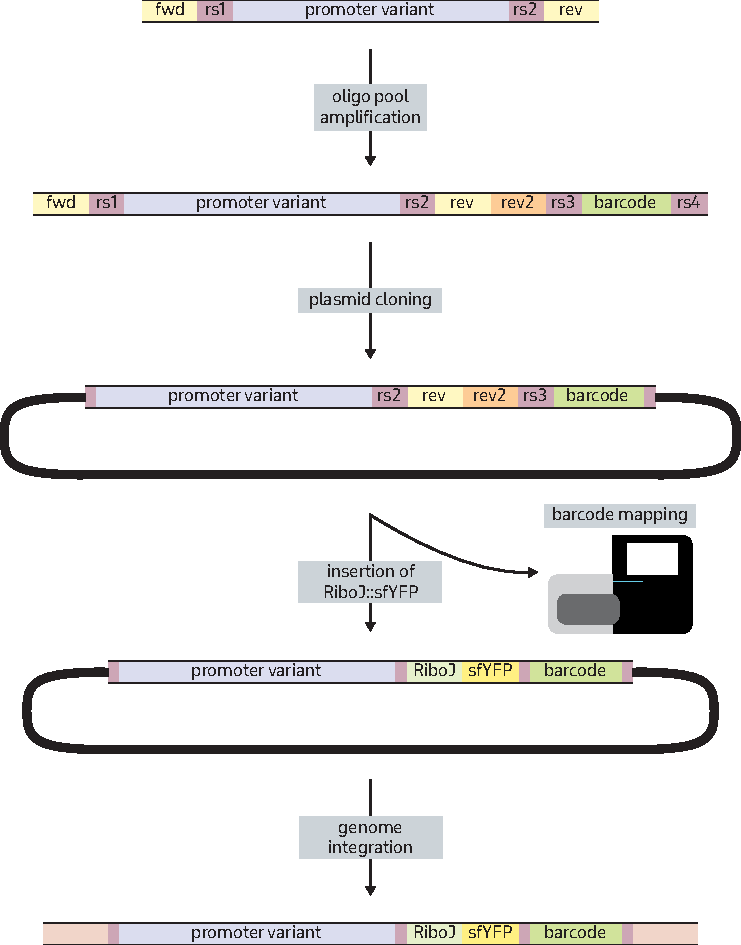
\includegraphics{../figures/cloning_scheme.pdf}
    \caption{Placeholder figure for cloning scheme.}
    \label{fig:cloning}
\end{figure}

\begin{figure}
    \centering
    \includegraphics[scale=1]{../figures/gc_content_first_6.pdf}
    \caption{}
    \label{fig:prom_gc_content}
\end{figure}
  